\subsection{Neural Systems Relevant to Memory and Sleep}

The neurobiology relevant to Targeted Memory Reactivation (TMR) is distributed
across interacting memory, sensory, and sleep-regulatory systems. For the present
translation problem, the critical issue is not a complete account of human
neuroanatomy, but the relationship among three functions: the encoding and
reactivation of recently acquired memories, the regulation of sensory access
during sleep, and the maintenance of physiological states in which consolidation
can occur. These functions depend principally on hippocampal--neocortical,
thalamocortical, and sleep--wake regulatory networks
\citep{squire2015consolidation,scammell2017sleep}.

The hippocampus and distributed neocortical networks occupy complementary roles
in declarative memory. During learning, the hippocampus rapidly binds distributed
features of an experience represented across cortical regions, allowing recently
acquired information to be retrieved as an integrated memory. Over time,
reactivation of hippocampal--cortical representations is thought to contribute
to systems-level reorganization and integration with existing cortical knowledge
\citep{squire2015consolidation,dudai2015consolidation}. This process should not
be interpreted as a simple transfer from a temporary hippocampal store to a
permanent cortical store. The degree to which long-term memories become
independent of the hippocampus varies across memory types and remains the subject
of theoretical and empirical debate. For TMR, the important point is narrower:
recent memories can remain susceptible to post-encoding modification through
reactivation of distributed representations.

Sleep also changes how these memory systems interact with incoming sensory
information. The thalamus participates in state-dependent regulation of
thalamocortical communication and contributes directly to characteristic NREM
oscillations, particularly sleep spindles. Sensory transmission is attenuated
and reorganized during sleep rather than completely blocked, allowing the brain
to reduce responsiveness to much of the external environment while retaining
the capacity to process selected stimuli
\citep{scammell2017sleep,fernandez2020spindles}. This partial sensory
accessibility is essential to the biological plausibility of TMR: an external
cue must influence ongoing neural processing without producing sufficient
activation to destabilize sleep.

Hypothalamic and brainstem circuits contribute to the regulation and stability
of sleep--wake states, while structures including the amygdala can modulate the
salience and persistence of particular memories. These systems are relevant to
TMR primarily because they influence the physiological state in which cueing
occurs and the probability that sensory stimulation produces arousal rather
than memory-related processing. They are therefore treated here as modulatory
components of a larger network rather than as independent memory-storage systems
\citep{scammell2017sleep}.

\begin{figure*}[t]
    \centering
    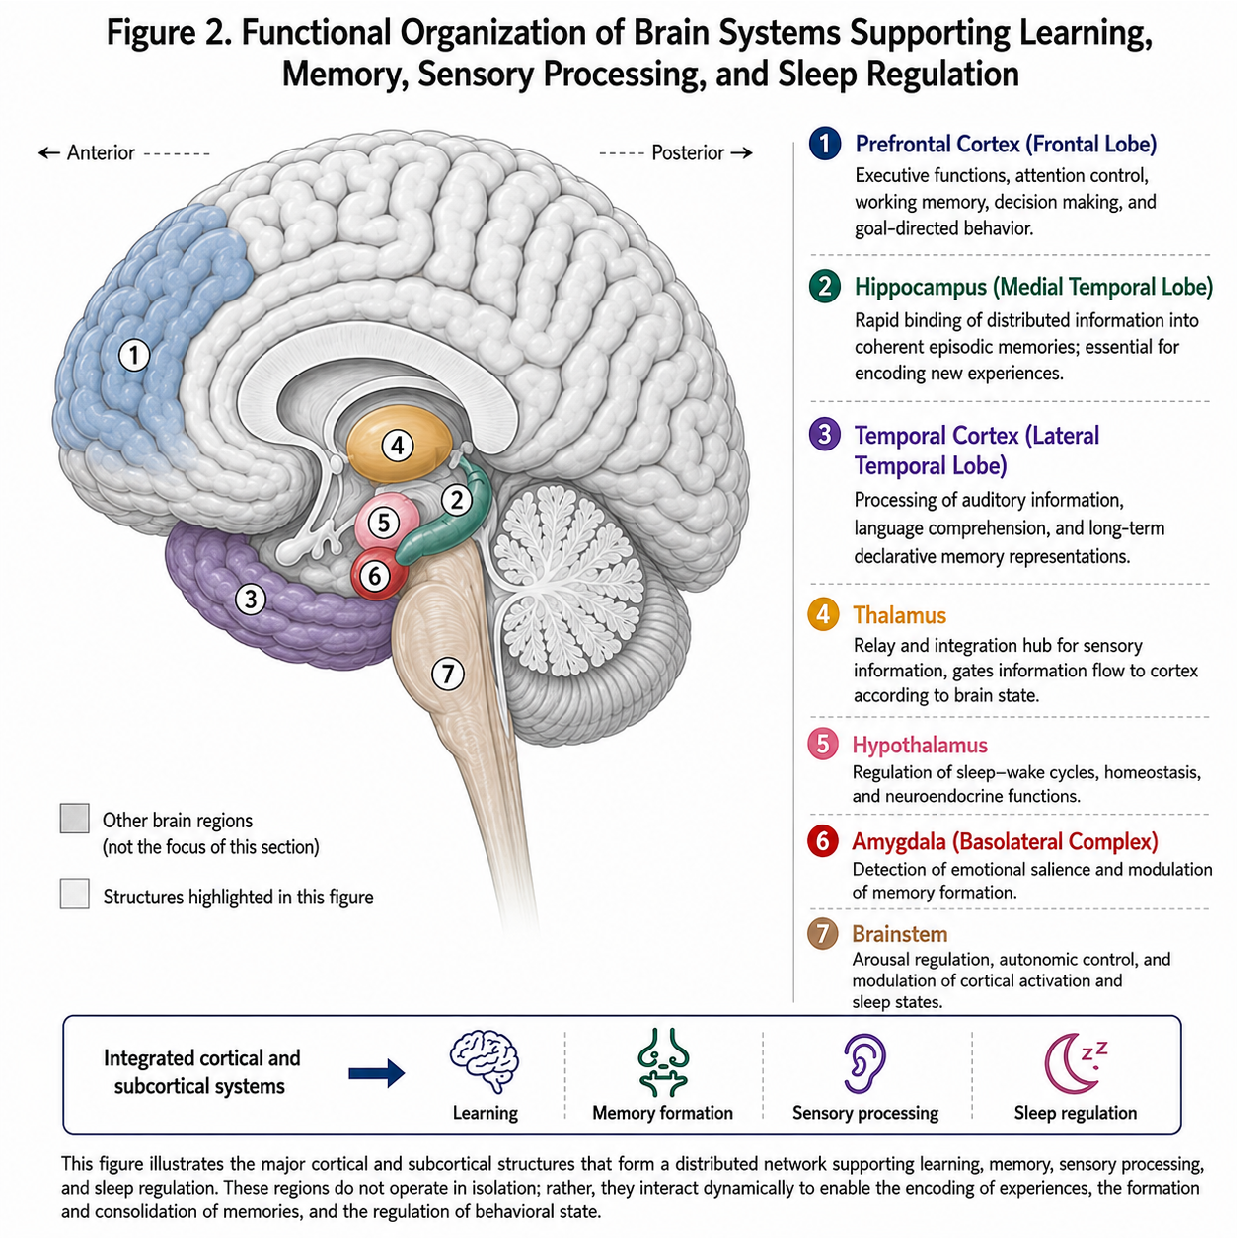
\includegraphics[width=\textwidth]
    {figures/fig2_memory_systems.pdf}
    \caption{
    Functional neural systems relevant to sleep-dependent memory processing.
    Hippocampal and distributed cortical networks support the encoding,
    reactivation, and longer-term reorganization of memory representations;
    thalamocortical circuits regulate state-dependent sensory processing and
    contribute to NREM oscillations; and hypothalamic and brainstem systems
    participate in sleep--wake and arousal regulation. The amygdala can
    additionally modulate memory according to emotional salience. The diagram
    represents a conceptual systems-level synthesis rather than anatomically
    independent functional modules
    \citep{squire2015consolidation,scammell2017sleep}.
    }
    \label{fig:functional_brain_systems}
\end{figure*}


\subsection{Electrophysiological Basis of Brain-State Monitoring}

For closed-loop TMR, the relevant bridge between neural physiology and
engineering is population-level electrophysiology. Information is transmitted
within and between neurons through electrical and chemical mechanisms, but
scalp-level measurements do not resolve individual neuronal communication.
Instead, coordinated activity across neuronal populations generates
extracellular electrical fields whose temporal structure can be measured at
progressively larger spatial scales.

Neural oscillations are recurring patterns of population activity produced by
interactions within and between neuronal circuits. They span multiple
frequencies and can organize the timing of neuronal excitability,
communication, and plasticity \citep{buzsaki2004oscillations}. Frequency bands
should not, however, be interpreted as one-to-one labels for specific cognitive
states. Multiple rhythms coexist, their properties vary across brain regions
and individuals, and their functional significance depends on the surrounding
physiological context. During sleep, several oscillatory events become
particularly informative because their occurrence and temporal relationships
change systematically across sleep states.

Electroencephalography (EEG) provides a non-invasive measurement of voltage
differences generated by these large-scale electrophysiological processes.
Scalp EEG is influenced primarily by coordinated transmembrane currents in
neuronal populations, particularly synaptic currents in spatially organized
cortical neurons, rather than by direct recording of individual action
potentials \citep{buzsaki2012origin}. EEG consequently provides high temporal
resolution but limited spatial specificity: it can reveal when large-scale
electrophysiological patterns occur without uniquely identifying the underlying
neuronal sources.

This distinction is important when EEG is used for sleep monitoring.
Conventional clinical sleep staging is based on polysomnography (PSG), which
combines EEG with electrooculography (EOG), electromyography (EMG), and other
physiological channels. Standard scoring assigns wake, N1, N2, N3, and REM
labels to successive epochs using characteristic combinations of these signals
\citep{silber2007scoring}. EEG contributes strongly to this classification,
particularly through changes in spectral activity and the appearance of events
such as K-complexes, sleep spindles, and slow waves, whereas rapid eye
movements are measured primarily by EOG and the reduction of skeletal-muscle
tone characteristic of REM sleep is assessed using EMG.

Conventional sleep-stage labels and the underlying electrophysiological events
also operate at different temporal scales. Manual staging is conventionally
performed over 30-s epochs, whereas slow waves, spindles, arousals, and other
transient events evolve over substantially shorter intervals
\citep{silber2007scoring}. A real-time intervention may therefore require more
than reproduction of conventional retrospective stage labels; it may also
require access to the continuous signal from which intervention-relevant events
and state transitions can be detected.

A further measurement boundary is particularly important for the later
engineering analysis. Cortical slow waves and sleep spindles are observable in
scalp EEG, whereas hippocampal sharp-wave ripples are primarily characterized
through intracranial recordings and are not directly available from ordinary
wearable scalp EEG. Human intracranial studies nevertheless show temporal
coordination among hippocampal ripples, sleep spindles, and slow oscillations
\citep{staresina2015nesting}. Accordingly, hippocampal ripple activity can
inform the biological model of sleep-dependent consolidation without being
treated as a directly measurable control signal in a first-generation wearable
EEG system.

\begin{figure*}[t]
    \centering
    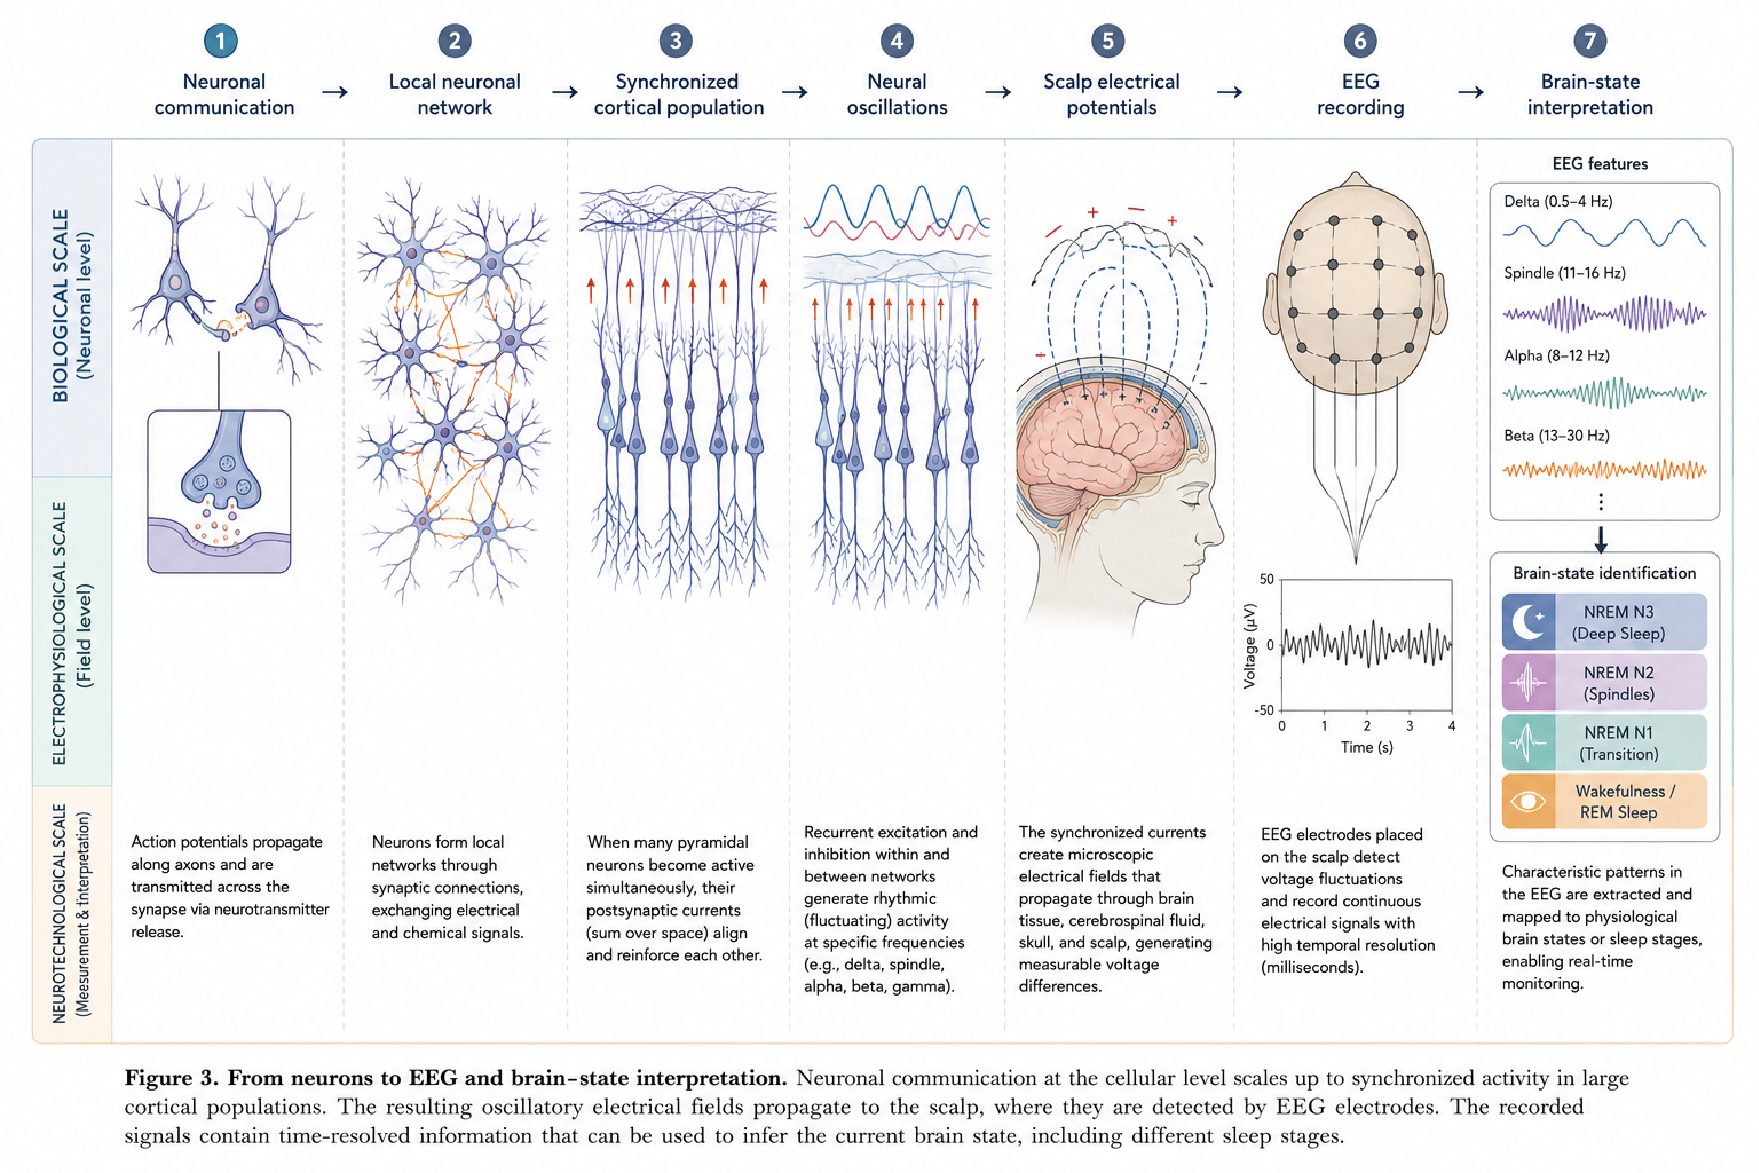
\includegraphics[width=\textwidth]
    {figures/fig3_neurons_to_EEG.pdf}
    \caption{
    Conceptual relationship between neuronal population activity and
    EEG-based brain-state interpretation. Coordinated transmembrane currents
    across neuronal populations generate extracellular fields that contribute
    to measurable scalp potentials. Their temporal organization produces EEG
    features, including oscillatory activity and transient events, that can be
    used as physiological indicators of sleep state. Scalp EEG reflects
    population-level activity and does not directly record individual neurons
    or deep hippocampal sharp-wave ripples
    \citep{buzsaki2012origin}.
    }
    \label{fig:neurons-to-eeg}
\end{figure*}


\subsection{Memory Consolidation and Reactivation}

Encoding does not immediately produce a fixed long-term memory. Newly acquired
representations remain susceptible to interference and modification, and their
persistence depends on biological processes collectively described as memory
consolidation. Consolidation operates across multiple temporal and spatial
scales, from cellular and synaptic modifications within initially engaged
circuits to systems-level changes in how memories are represented across
hippocampal and cortical networks
\citep{squire2015consolidation,dudai2015consolidation}.

Synaptic consolidation refers broadly to post-learning cellular processes that
stabilize experience-dependent changes within local circuits. Systems
consolidation concerns longer-term reorganization of distributed memory
representations and changes in interactions between the hippocampus and
neocortex. These processes should not be treated as a single linear transfer
mechanism: their time courses overlap, their expression depends on the type of
memory, and multiple theoretical accounts differ in the extent to which remote
memories continue to require hippocampal involvement
\citep{squire2015consolidation,dudai2015consolidation}.

A central process linking learning to later systems-level change is memory
reactivation. Neural patterns related to previous experience can reappear after
encoding during both wakefulness and sleep. During NREM sleep, such
reactivation is frequently observed in temporal association with hippocampal
sharp-wave ripples and with cortical and thalamocortical oscillations implicated
in memory processing \citep{rasch2013sleep,klinzing2019mechanisms}. Reactivation
is therefore widely considered an important component of contemporary models
of sleep-dependent systems consolidation.

The mechanistic interpretation nevertheless requires caution. Reactivation is
not synonymous with consolidation, and the occurrence of replay-like activity
does not imply that every reactivation event strengthens a memory. Instead,
reactivation provides an opportunity for previously encoded representations to
be modified, integrated, or stabilized under physiological conditions that
support plasticity. The behavioral consequences depend on the memory,
surrounding neural state, and temporal organization of the relevant activity
\citep{dudai2015consolidation,klinzing2019mechanisms}.

This distinction is central to TMR. A sensory cue presented during sleep cannot
be assumed to create or restore a memory that was not successfully encoded.
Rather, TMR depends on an association established during wakefulness and seeks
to bias subsequent reactivation toward the corresponding representation. The
scientific target of the intervention is therefore an endogenous post-encoding
process, not memory formation independently of prior learning.


\subsection{Sleep Architecture and Oscillatory Coordination of Memory}

Human sleep is organized into recurring transitions among NREM and REM states.
Under contemporary clinical scoring conventions, NREM sleep is divided into
N1, N2, and N3. N1 represents the transition from wakefulness into sleep; N2 is
characterized in part by K-complexes and sleep spindles; and N3 contains
prominent high-amplitude slow-wave activity and is commonly referred to as
slow-wave sleep (SWS) in human experimental research. REM sleep differs from
NREM sleep through a combination of relatively low-amplitude mixed-frequency
EEG activity, rapid eye movements, and reduced skeletal-muscle tone
\citep{silber2007scoring}.

These stages should not be interpreted as discrete functional compartments in
which a single cognitive process occurs exclusively. Memory-related processing
is distributed across the sleep period, and different forms of learning can
show different relationships with NREM and REM physiology
\citep{diekelmann2010memory,rasch2013sleep}. For the declarative memory
processes most relevant to much of the TMR literature, NREM sleep---particularly
N2 and N3---provides a well-supported physiological context for examining
reactivation and hippocampal--neocortical communication. This does not imply
that N3 is universally optimal for every memory domain or cueing protocol.

A prominent mechanistic framework for NREM-dependent systems consolidation
centers on the temporal coordination of cortical slow oscillations,
thalamocortical sleep spindles, and hippocampal sharp-wave ripples. Slow
oscillations organize alternating periods of cortical excitability; spindles
emerge from thalamocortical circuitry and are associated with transient windows
of cortical plasticity; and hippocampal sharp-wave ripples are closely
associated with replay of recently experienced activity. Converging evidence
suggests that their temporal nesting can support communication between
hippocampal and cortical memory systems
\citep{staresina2015nesting,fernandez2020spindles,klinzing2019mechanisms}.

The coupling of these events is scientifically important but should not be
converted prematurely into a requirement for phase-specific stimulation.
Evidence that oscillatory coordination contributes to consolidation does not,
by itself, establish that a first-generation TMR system must detect every event
or deliver cues at a particular oscillatory phase. Stage-aware cueing and
event- or phase-aware cueing therefore represent distinct levels of
intervention control. Whether the additional temporal precision of the latter
produces a reproducible behavioral advantage is an empirical question addressed
later in the translational analysis.

For wearable implementation, this distinction also separates the biological
mechanism from what can actually be observed. Scalp EEG can provide information
about sleep stage, cortical slow-wave activity, and sleep spindles, while deeper
hippocampal processes remain indirectly inferred. The relevant engineering
question is consequently not whether every component of the consolidation
mechanism can be measured non-invasively, but whether the observable signals
provide sufficient information to identify physiologically appropriate
conditions for intervention.

\begin{figure*}[t]
    \centering
    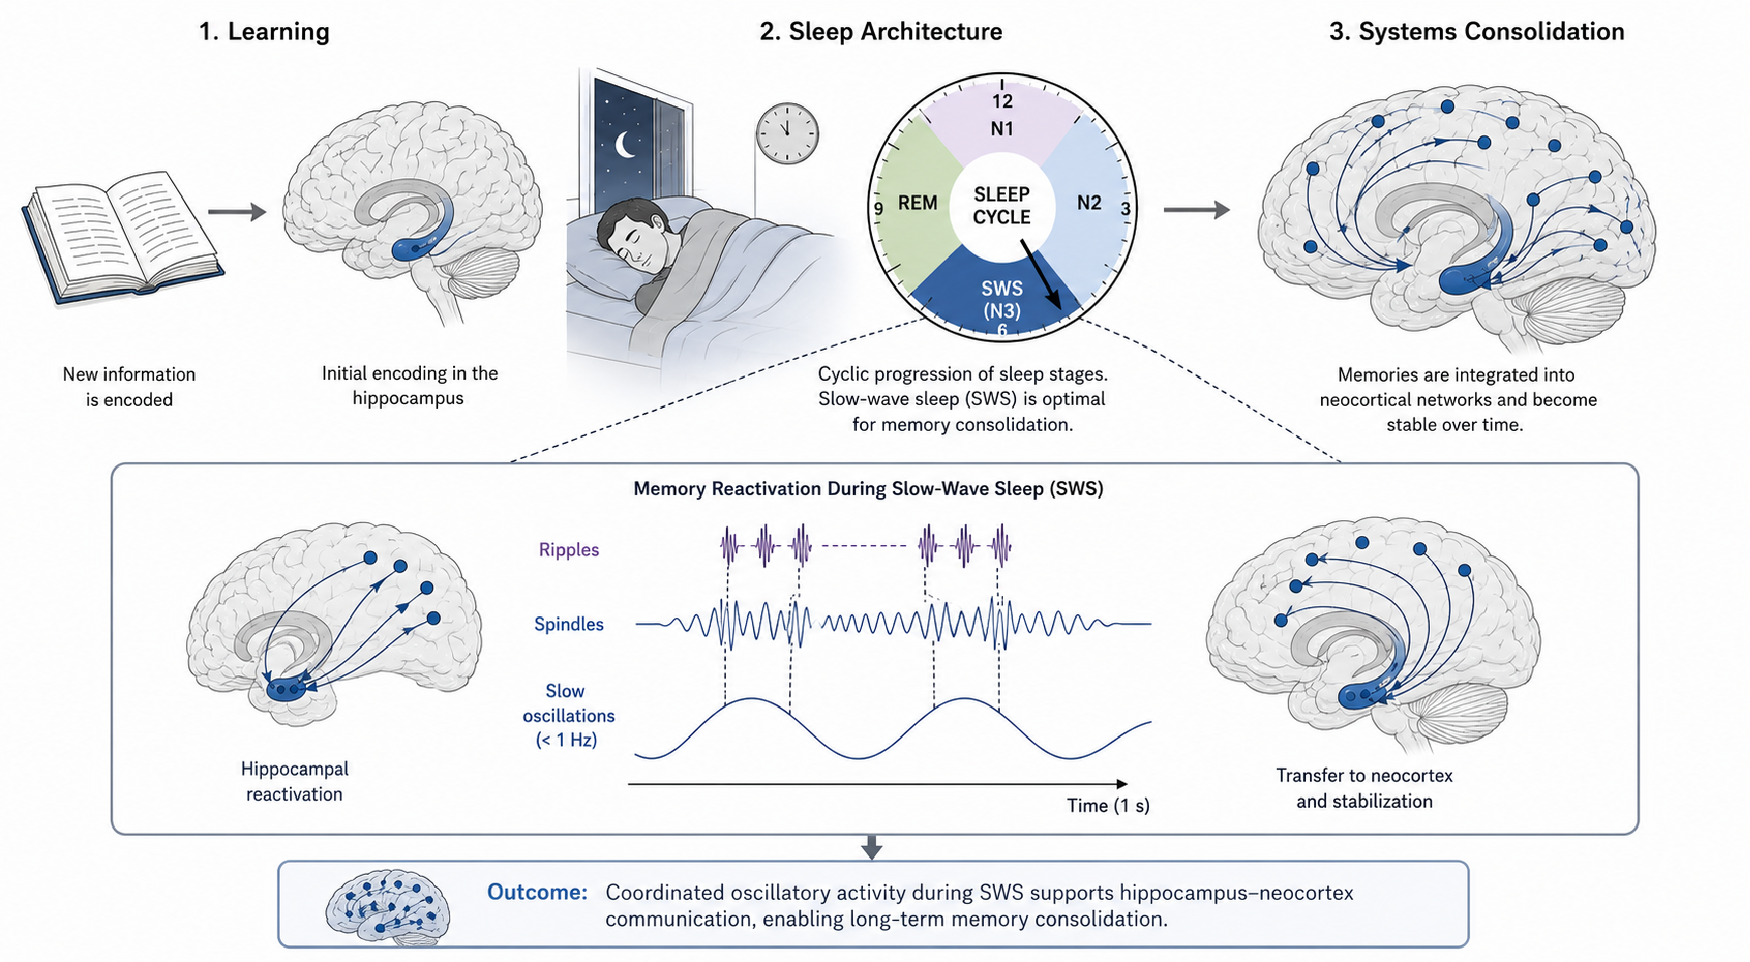
\includegraphics[width=\textwidth]
    {figures/fig4_sleep_dependent_consolidation.pdf}
    \caption{
    Conceptual framework of sleep-dependent systems memory consolidation.
    Recently encoded memories initially depend strongly on interactions between
    hippocampal and distributed cortical representations. During NREM sleep,
    memory reactivation occurs within a physiological environment characterized
    by coordinated cortical slow oscillations, thalamocortical sleep spindles,
    and hippocampal sharp-wave ripples. Their temporal interaction is proposed
    to support communication and longer-term reorganization across memory
    networks. The figure represents a mechanistic synthesis rather than a
    claim that consolidation proceeds through a single deterministic pathway
    \citep{rasch2013sleep,staresina2015nesting,klinzing2019mechanisms}.
    }
    \label{fig:sleep-dependent-consolidation}
\end{figure*}

Together, these findings establish the biological constraints relevant to TMR:
a previously encoded representation must remain capable of reactivation, cueing
must occur within an appropriate physiological state, and the intervention must
preserve rather than disrupt the sleep processes associated with consolidation.
Section~4 examines the extent to which experimental TMR can exploit these
conditions to produce measurable changes in subsequent memory.